\documentclass[a4paper,ngerman]{scrartcl}

\usepackage{amsmath}
\usepackage{amsfonts}
\usepackage{amssymb}
\usepackage[utf8]{inputenc}
\usepackage{graphicx}
\usepackage[ngerman]{babel}
\usepackage{hyperref}
\usepackage{float}
\usepackage{caption}
\usepackage{subcaption}
\usepackage{multirow}  %for tables
\usepackage{icomma} % Handle german comma as decimal point in numbers
\usepackage{units,siunitx} % Write units with correct spacing
\usepackage{upgreek} % provide non-italic greek letters
\usepackage{url}
\usepackage{booktabs}
\usepackage{placeins}
%\usepackage{subfig}

% Formatting of table & figure captions
\captionsetup{font={sf,footnotesize},labelfont=bf,textfont=sl,skip=6pt}

%locale for units to german
\sisetup{locale = DE}
\sisetup{separate-uncertainty=true}

\setlength{\abovecaptionskip}{6pt}
\setlength{\belowcaptionskip}{0pt}

\title{Magnetisierung}
\date{\today}
\author{Michel Rausch, Michael Eliachevitch}

\begin{document}

\maketitle
\tableofcontents
\newpage

\section{Versuchsvorbereitung}

\subsection{Einleitung}

%Versuchsbeschreibung:
%Es wird die Magnetisierung von Selten-Erd-Metallen (Tb, Gd)im Temperaturbereich T = 77 - 300 K bestimmt. 
%Dazu wird ein supraleitendes Quanteninterferometer (Superconducting Quantum-Interference Device, SQUID) aus einem Hochtemperatursupraleiter verwendet, das sich in einem Flüssigkstickstoff-gekühlten Dewar befindet.

Mit einem supraleitendem Quanteninterferometer, einem sogenanntem
"`superconducting quantum interference device"' (SQUID), soll
die Magnetisierung der Seltenen-Erde-Metalle Terbium (Tb) und
Gadolinium (SQUID) über einen Temperaturbereich von 
$\SI{77}{\kelvin} < T < \SI{300}{\kelvin}$ bestimmt werden.
Das SQUID wird mit flüssigem Stickstoff gekühlt und befindet sich
daher in einem Dewar. In diesem Versuch werden die Grundlagen der
Supraleitfähigkeit und Magnetisierung vertieft und in einer Messung
angewandt.


\subsection{Theoretische Grundlagen}

\subsubsection{Supraleitung}

Supraleitung bezeichnet den Effekt, das einige Materialien,
insbesondere Metalle, bei Unterschreitung einer Grenztemperatur
$T_{\mathrm{C}}$, die bei metallischen Supraleitern meist im Bereich
weniger Kelvin liegt, ihren elektrischen Widerstand verlieren.
Dies wird durch die Bildung von sogenannten Cooper-Paaren erklärt,
wobei jeweils zwei Elektronen Zustände mit ganzzahligem
Spin bilden, die durch ein Pseudoteilchen beschrieben werden können,
bei dem es sich um ein Boson handelt.


Sogenannte Hochtemperatursupraleiter, die meist aus Keramiken
bestehen, werden bereits bei Temperaturen von flüssigem Stickstoff
supraleitend.
Jedoch können sie nicht mit Hilfe von Cooperpaaren erklärt werden.  


\paragraph{Supraleiter in Magnetfeldern:
}
Im supraleitenden Zustand wird das Material diamagnetisch und
Magnetfelder können nicht, oder nur gequantelt, in den Supraleiter
dringen. 
Bei Supraleitern 1. Art werden vorhandene Magnetfelder verdrängt im
supraleitenden Zustand vollständig verdrängt, was durch Abschirmströme
geschieht. 
Das passiert sowohl wenn der supraleitende Zustand im vorhanden
Magnetfeld erreicht wird als auch, wenn ein Supraleiter in ein
Magnetfeld gebracht wird. Das bezeichnet man als
Meißner-Ochsenfeld-Effekt.
Sobald der Magnetische Fluss eine kritische Größe überschreitet,
also $B > B_C$, bricht die Supraleitung zusammen.

Supraleiter 2. Art verhalten sich bei in einem Bereich $B < B_{C1}$
wie Supraleiter 1. Art und verdrängen alle Magnetfelder durch
Abschirmströme. 
In einem Bereich $B_{C1} < B < B_{C2}$ jedoch lassen sie jedoch selbst
im supraleitenden Zustand einen magnetischen Fluss durch $\Phi$, wobei
dieser nur gequantelt auftritt,
da es sich um ein quantenmechanisches System mit Randbedingungen
handelt. Die Quantisierung ist dabei gegeben durch den elementaren
magnetischen Flussquant

\begin{equation}
  \label{eq:phi0}
  \Phi_0 = \frac{h}{2 e} = \SI{2e-15}{\volt\second}~.
\end{equation},

Anschaulich vorstellen lässt sich das so, 
dass der magnetische Fluss die
supraleitende Schlaufe in kleinen "`Tunneln"' dieser Größe durchquert.


Bei Flussdichten $B > B_{C2}$ bricht auch bei Supraleitern 2. Art die
Supraleitung zusammen.


\paragraph{Josephson-Effekt:} Unter den Josephson-Effekten fasst man
zwei weitere nur quantenmechanisch erklärbare, makroskopische
Eigenschaften von Supraleitern zusammen. 
Sie treten auf, wenn man zwei Supraleiter durch eine dünne
isolierende (\emph{SIS}) oder normalleitende
Schicht (\emph{SNS}) voneinander trennt,
die man oft als \emph{Schwachstelle} bezeichnet. 
Dennoch kann, ohne dass die Supraleitung zusammenbricht, Strom durch die Grenzschicht fließen, da es zu einem
quantenmechanischen Tunneln von Cooper-Paaren durch die Grenzschicht kommt.


% ...

% \begin{figure}[tb!]
% \centering
% 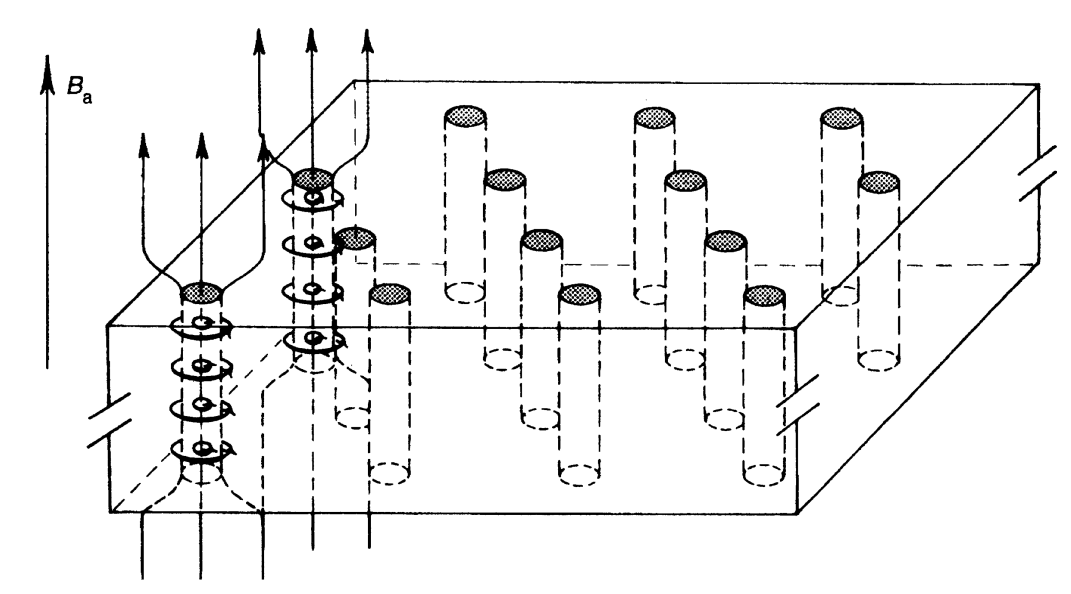
\includegraphics[width=0.7\textwidth]{abbildungen/typ2_supraleiter.png}
% \caption[Versuchsplatz]{\textbf{Flussfadengitter in einem Typ II-Supraleiter [\ref{ref:mappe}].} Magnetfelder treten durch Kanäle in den Supraleiter ein. Die Flüsse sind quantisiert und verlaufen entlang der Magnetfeldrichtung.}
% \label{fig:typII}
% \end{figure}


% \subsubsection{YBCO}

% Der Supraleiter Yttrium-Barium-Kupferoxid $\mathrm{YBa}_2 \mathrm{Cu}_3 \mathrm{O}_{7-x}$ (\textbf{YBCO}) ist ein Hochtemperatursupraleiter.
% Die kritische Temperatur beträgt 
% \begin{equation}
% T_\mathrm{C} = \SI{93}{K} ~.
% \end{equation}
% Es ist ein harter Supraleiter zweiter Art, der Flussfäden fest einfriert.
% Die Kristallstruktur ist Perowskitartig und abhängig von einer wohlgeordneten Struktur.

\FloatBarrier
\subsubsection{Funktionsweise eines RF-SQUIDs}
Ein sogenanntes SQUID (\emph{superconducting quantum interference device}) 
ist ein Gerät zur Detektion von kleinsten Änderungen in
magnetischen Feldern. 
Hier werden wir ein  in diesem Versuch verwendetes, sogenanntes RF-SQUID beschreiben, 
das mit einem Wechselstrom betrieben wird.
Es besteht aus einem supraleitenden Ring, der eine dünne, nicht-supraleitende Schwachstelle besitzt. 
Gerät das SQUID nun in ein externes Magnetfeld,
so wird in dem Ring ein Kompensationsstrom induziert,
der den magnetischen Fluss durch den Ring auf ein ganzzahliges 
Vielfaches des Flussquants $\Phi_0$ reduziert oder erhöht.

Bei Änderungen des äußeren Magnetfeldes um mehr als ein Flussquant übersteigt der Kompensationsstrom beim SQUID eine kritische Stromdichte und die Supraleitung bricht zusammen, 
sodass der Strom wieder durch Elektronen getragen wird und es zu 
Energieverlusten kommt.

Ein RF-SQUID ist induktiv an ein Wechselfeld gekoppelt, 
meist mit einer Frequenz von einigen 100\,MHz,
mit welchem durch Wechselfelder in Resonanz ein externer Wechselstrom in dem SQUID induziert wird, welcher den Kompensationsstrom überlagert, sodass es periodisch zwischen dem supraleitenden Zustand und dem normalleitenden Zustand, bei dem Energie verbraucht wird, 
hin und her wechselt. 
Die verbrauchte Energie wird dabei dem Schwingkreis entnommen,
der dadurch gedämpft wird, sodass an ihm die Spannungsamplitude abnimmt. 
Aus dieser Spannungsänderung kann dann die Änderung des Magnetfeldes bestimmt werden.
Da man in der Praxis meist mit Magnetfeldern arbeitet, 
die deutlich größer sind als ein Flussquant, 
muss das SQUID als Nulldetektor betrieben werden,
indem man externe Feldänderungen mit einer Spule ausgleicht,
die mit einem Gegenkopplungs-Gleichstrom betrieben wird. 
Dieser ist proportional zu externen Feldänderungen, welche damit nun in einem großen Bereich bestimmt werden können.


In unserem Versuch wird ein 
SQUID der Firma \emph{Jülicher SQUID GmbH} verwendet,
das auf dem Hochtemperatursupraleiter
Yttrium-Barium-Kupferoxid (\emph{YBCO}) mit einer kritischen
Temperatur $T_\mathrm{C} = \SI{93}{K}$ basiert.

\section{Versuchsauswertung}



\subsection{Kalibrierung des SQUIDs}


\subsubsection*{Mit der Kalibrierungsspule}

Ein Kupferzylinder ($\rm{Durchmesser} = \SI{0.7}{\centi \meter}$,  Höhe $ = \SI{0.7}{\centi \meter}$) mit der Spule wurde auf den Probenhalter geschraubt. 
Der Halter wurde so im Magnetfeld platziert, dass die Spule nach oben gerichtet war.
Damit wurde sichergestellt, dass die Proben später in einer möglichst gleichen und somit vergleichbaren Position befanden.
Zehn Messwerte wurden genommen, für unterschiedliche Spulenströme. 
Diese sind in Tabelle \ref{tab:Kalibrierung-Magnetfeld} aufgelistet.
Das Magnetfeld des SQUIDs wurde nach dem Biot-Savartschem Gesetz [\ref{ref:mappe}] berechnet mit

\begin{equation}
B_{\mathrm{Spule}} = \mu_{\rm{0}} \cdot \frac{R^2}{2 x^3} ~,
\end{equation}

mit  der absoluten magnetischen Permeabilität $\mu_{\rm{0}}$, dem Abstand der Spule zum SQUID $d = \SI{1.4}{\centi \meter}$ und dem Radius der Spule $R = \SI{0.35}{\centi \meter} $.
Der Abstand der Spule zum SQUID schien beim tatsächlichem Aufbau
deutlich größer zu sein, als in der Versuchsbeschreibung
angegeben,
dennoch wurde mit dem Wert aus der Mappe gerechnet.


\begin{table}[tb!]
\centering
\caption[Kalibrierung]{\textbf{Messwerte zur Kalibrierung des SQUIDs.} }
\begin{tabular}{ccc}
\toprule
Spulenstrom	in mA &	SQUID-Spannung in mV	\\
\midrule
0	&	19	\\
40	&	27	\\
80	&	29	\\
119	&	42	\\
147	&	42	\\
180	&	52	\\
209	&	40	\\
235	&	65	\\
315	&	58	\\
360	&	66	\\
\bottomrule
\end{tabular}
\label{tab:Kalibrierung-Magnetfeld}
\end{table}

In Abbildung \ref{fig:Kalibrierung-Magnetfeld} ist die Messreihe mit
zugehörigem linearen Fit dargestellt, der mit dem Python-Modul
\emph{scipy} erstellt wurde.
Man erkennt, dass sehr geringe Magnetfeldstärken in der Größenordnung eines Mikroteslas gemessen wurden.
Das SQUID ist also ein äußerst empfindliches Messgerät.
Die lineare Regression ergab

\begin{equation}
\label{eq:B(U_SQUID)}
B = \SI{18+-3}{\micro \tesla \per \mV} \cdot U_{\mathrm{SQUID}} - \SI{0.3+-0.1}{\micro \tesla} ~.
\end{equation}

%U_{\mathrm{SQUID}} = \SI{46+-7}{\mV \per \micro \tesla} \cdot B + \SI{22+-4}{\mV} ~.

\begin{figure}
\centering
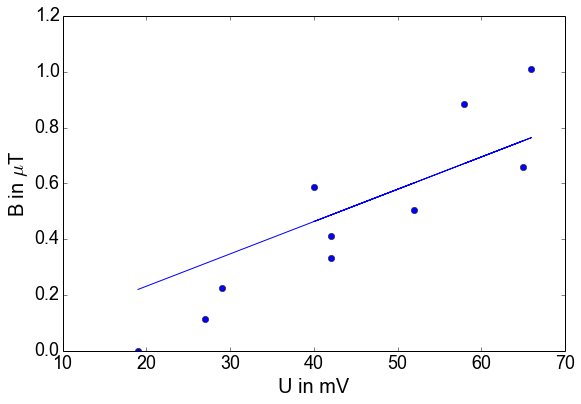
\includegraphics[width=0.8\textwidth]{abbildungen/kalibrierung_spule.png}
\caption[Kalibrierung des SQUIDs mit Spule]{\textbf{Kalibrierung des SQUIDs mit Spule.} Für unterschiedliche Ströme durch die Spule wurde die resultierende Spannung am SQUID gemessen. Die Messwerte streuten stark, daher war ein hoher Fehler zu erwarten.}
\label{fig:Kalibrierung-Magnetfeld}
\end{figure}




\subsubsection*{Mit der Nickelprobe}

Eine Nickelprobe mit dem Ausmaßen $\SI{5}{\mm} \times \SI{5}{\mm} \times \SI{0.1}{\mm}$ wurde auf den Probenhalter geschraubt.
Aus ihrem Volumen und der spezifischen Magnetisierung von Nickel [\ref{ref:mappe}]
\begin{equation}
\sigma = \SI{55.09}{\ampere \square \meter \per \kg} ~,
\end{equation}
sowie der Masse der Probe 
\begin{equation}
m = \SI{0.0202}{\gram} ~,
\end{equation}
wurde das maximale magnetische Moment der Nickelprobe 

\begin{equation}
\mu_{\mathrm{Ni}} = \SI{1.11}{\mA \square \meter}
\end{equation}

bestimmt. Die Probe wurde magnetisiert, bei einem maximalem Strom durch die Magnetspulen von
\begin{equation}
I_{\mathrm{Spule}} = \SI{1.168}{\ampere} ~.
\end{equation}

Einmal wurde die Probe senkrecht zum Magnetfeld orientiert, das andere Mal parallel.
Bei einer senkrechten Orientierung betrug die Spannung am SQUID ohne Probe 
\begin{equation}
U_{\mathrm{ohne Probe},\perp} = \SI{83}{mV} ~.
\end{equation}
Mit der Probe stieg die Spannung auf
\begin{equation}
U_{\mathrm{mit Probe},\perp} = \SI{970}{mV} ~.
\end{equation}

Die Spannungsdifferenz wird durch die Probe verursacht und wird in 
Gleichung \eqref{eq:B(U_SQUID)} als Argument verwendet, um das Magnetfeld zu bestimmen. 

\begin{equation}
B_{\mathrm{mit Probe},\perp} = \SI{16+-3}{mT} ~.
\end{equation}


Als die Probe parallel zum Magnetfeld war ergaben sich analog
\begin{equation}
U_{\mathrm{ohne Probe},\parallel} = \SI{70}{mV} ~,
\end{equation}
\begin{equation}
U_{\mathrm{mit Probe},\parallel} = \SI{1620}{mV} ~,
\end{equation}
\begin{equation}
B_{\parallel} = \SI{28+-5}{mT} ~.
\end{equation}

Im Vergleich sieht man, dass die Nickelprobe bei parallelem Einbau stärker magnetisiert worden ist.
Für das Magnetfeld gilt mit dem Abstand der probe zum SQUID [\ref{ref:mappe}]
\begin{equation}
B = \frac{\mu_{\rm{0}} \mu }{2 \uppi x^3} ~.
\end{equation}

Daraus folgt
\begin{equation}
\label{eq:mu(B))}
\mu = \frac{2 \uppi B x^3 }{\mu_{\rm{0}}} ~.
\end{equation}

Die Magnetischen Momente sind dann für den senkrechten Einbau
\begin{equation}
\mu_{\perp} = \SI{0.22+-0.04}{\mA \square \meter} ~,
\end{equation}

und für den parallelen
\begin{equation}
\mu_{\parallel} = \SI{0.38+-0.07}{\mA \square \meter} ~.
\end{equation}

In beiden Fällen ist das magnetische Moment, und somit die Magnetisierung, geringer als die maximal mögliche.
Dies ist mit der Stärke des Magnetfeldes zu erklären.
Das vorhandene Netzteil und die Spule konnten nur Magnetfeldstärken
liefern, die nicht zur Sättigung genügten.
Da die Probe nicht vollständig aufmagnetisiert wurde, kann von einem linearem Verhältnis der Magnetisierung zur Magnetfeldstärke ausgegangen werden.

Aus Gleichungen \eqref{eq:B(U_SQUID)} und \eqref{eq:mu(B))} zusammen folgt der Zusammenhang zwischen Magnetisierung und Spannung am SQUID

\begin{equation}
\label{eq:kalib}
\mu(U_{\mathrm{SQUID}}) = \frac{2 \uppi  x^3 }{\mu_{\rm{0}}} \cdot  \left( \SI{18+-3}{\micro \tesla \per \mV}  \cdot U_{\mathrm{SQUID}} - \SI{0.3+-0.1}{\micro \tesla} \right) ~.
\end{equation}

Die Kalibrierung der Spule war ungenau, daher war ein hoher statistischer Fehler zu erwarten.
Zudem war der Abstand der Probe zum SQUID wahrscheinlich größer als angegeben.
Das Verhalten der Probe unter einem Magnetfeld entspricht jedoch den Erwartungen. 

\subsection{Magnetisierungsmessungen}

\subsubsection{Terbiumprobe bei senkrechtem Einbau}

\subsubsection*{Messung mit im Nullfeld gekühlter Probe ohne Magnetisierung}

Die Probe wurde in die Spule montiert und abgekühlt.
Es wurde kein Magnetfeld angelegt.
Die Messung begann, als die Temperatur unter \SI{80}{K} gesunken war.
Die Probe wurde in das SQUID eingebaut und die Kühlung wurde unterbrochen.
Um den Aufwärmvorgang zu beschleunigen wurde Pressluft eingeleitet.
Die vorhandene Software protokollierte die Spannungen am SQUID und die zugehörige Temperatur.
In Abbildung \ref{fig:Tb_sr_0} ist die Messreihe gezeigt.


\begin{figure}
\centering
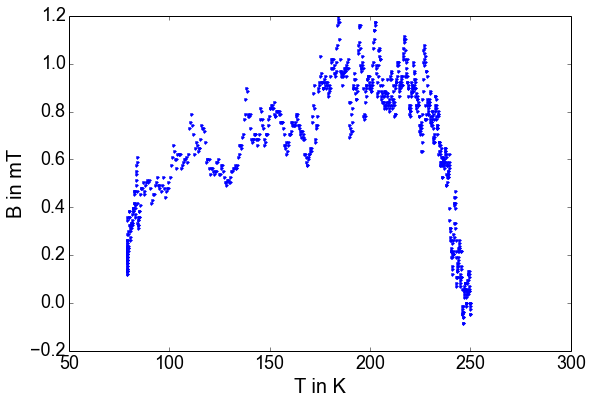
\includegraphics[width=0.6\textwidth]{abbildungen/Tb_sr_0.png}
\caption[Terbiumprobe senkrecht bei Nullfeld]{\textbf{Terbiumprobe senkrecht bei Nullfeld gekühlt, Rohdaten.} Das Magnetfeld am SQUID ist über die Temperatur aufgetragen.}
\label{fig:Tb_sr_0}
\end{figure}

Über einen Anteil von 10~\% wurde eine lokale Regression (LOWESS) durchgeführt, wie in Abbildung \ref{fig:Tb_sr_0_glatt} gezeigt ist.
Um die Curietemperatur zu bestimmen, wurde davon der Gradient gebildet.
Das sichtbare Minimum befindet sich an der Tempemit den ratur

\begin{equation}
T_{\rm{C}} = \SI{244}{\K} ~.
\end{equation}


\begin{figure}
\centering
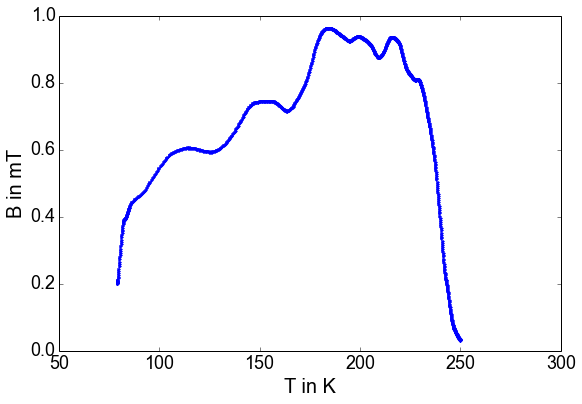
\includegraphics[width=0.5\textwidth]{abbildungen/Tb_sr_0_glatt.png}
\caption[Terbiumprobe senkrecht bei Nullfeld]{\textbf{Terbiumprobe bei
    senkrechtem Magnetfeld im Nullfeld gekühlt, geglättet mit LOWESS.}
  Das Magnetfeld am SQUID ist über die Temperatur aufgetragen, wie in
  Abb. \ref{fig:Tb_sr_0} zu sehen ist. Mit der Python-Funktion LOWESS
  aus dem Python-Moduls \emph{statsmodels} wurde eine lokale Regression über 10~\% der Daten durchgeführt.}
\label{fig:Tb_sr_0_glatt}
\end{figure}


\begin{figure}
\centering
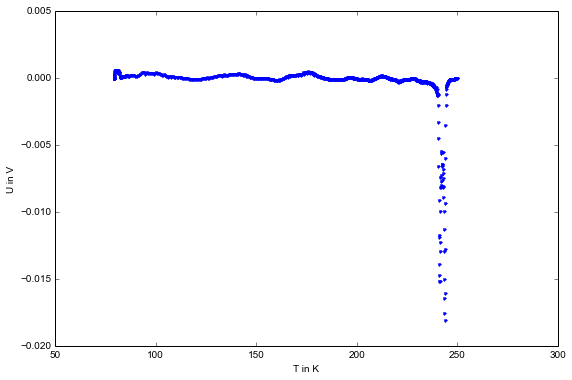
\includegraphics[width=0.6\textwidth]{abbildungen/Tb_sr_0_grad.png}
\caption[Terbiumprobe senkrecht bei Nullfeld]{\textbf{Terbiumprobe
    senkrechtem Magnetfeld im Nullfeld gekühlt, geglättet und Gradient gebildet.} 
    Die Steigung des Magnetfeldes am SQUID ist über die Temperatur aufgetragen. Ein Minimum ist an der Curietemperatur zu erkennen.}
\label{fig:Tb_sr_0_grad}
\end{figure}

\subsubsection*{Messung mit im Nullfeld gekühlter Probe mit Magnetisierung bei tiefer Temperatur und einem Magnetfeld mit \SI{15}{mT}}

Die Probe wurde nach dem Erwärmen wieder gekühlt auf unter \SI{80}{K}.
Dabei wurde kein Magnetfeld angelegt.
Erst als die Probe abgekühlt war, wurde an die Spule ein Strom angelegt, sodass ein Magnetfeld mit \SI{15}{mT} vorhanden war.
Der Strom durch die Spule betrug dabei etwa \SI{150}{\mA}.
Die Umrechnung vom Spulenstrom auf das Magnetfeld konnte mit 
\begin{equation}
10 \cdot B/\mathrm{mT} = I /\mathrm{mA}
\end{equation} 
genähert werden. 
Die Umrechnung war genauer gegeben, aber da sich der Strom nicht genau einstellen lies, konnte auf höhere Genauigkeit verzichtet werden.


\begin{figure}
\centering
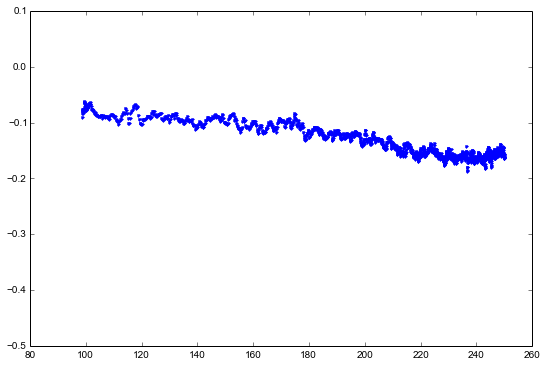
\includegraphics[width=0.6\textwidth]{abbildungen/Tb_sr_0_mit.png}
\caption[Terbiumprobe senkrecht bei Nullfeld]{\textbf{Terbiumprobe senkrecht bei Nullfeld gekühlt, Rohdaten.} Das Magnetfeld am SQUID ist über die Temperatur aufgetragen.}
\label{fig:Tb_sr_0_mit}
\end{figure}

Die Messergebnisse sind in Abbildung \ref{fig:Tb_sr_0_mit} gezeigt. 
Der Gradient wurde aus den geglätteten Daten gebildet, wie in Abbildung \ref{fig:Tb_sr_0_grad_mit} dargestellt ist. 
Es ist kein ausgewiesenes Minimum zu erkennen, daher konnte keine Curietemperatur bestimmt werden.


\begin{figure}
\centering
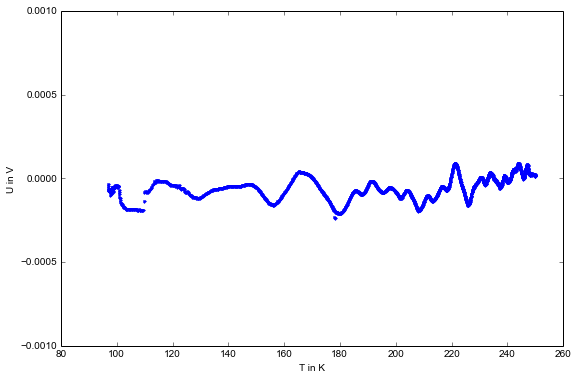
\includegraphics[width=0.6\textwidth]{abbildungen/Tb_sr_0_grad_mit.png}
\caption[Terbiumprobe senkrecht bei Nullfeld]{\textbf{Terbiumprobe senkrecht bei Nullfeld gekühlt, geglättet und Gradient gebildet} Das Die Steigung des Magnetfeldes ist über die Temperatur aufgetragen. Es wurden über über 25~\% der Daten mittels LOWESS geglättet. Es ist kein Minimum zu erkennen und somit keine Curietemperatur ermittelbar.}
\label{fig:Tb_sr_0_grad_mit}
\end{figure}



\subsubsection*{Messung mit im Feld gekühlter Probe bei \SI{15}{mT}}


Das Magnetfeld wurde angestellt, bevor die Kühlung begann. 
Die Probe wurde bei aktivem Magnetfeld gekühlt. 
Gemessen wurde wie vorhin beim Erwärmen.
Hier traten einige Sprünge auf, wie in Abbildung \ref{fig:Tb_sr_15} zu sehen ist. 
Die Sprünge wurden nach Augenmaß korrigiert, aber da viele Unstetigkeiten im interessanten Bereich um die Curietemperatur auftraten,
konnte die Curietemperatur nur schwer ermittelt werden.
Sie konnte dennoch identifiziert werden mit 

\begin{equation}
T_{\rm{C}} = \SI{235}{\K} ~.
\end{equation}


\begin{figure}
\centering
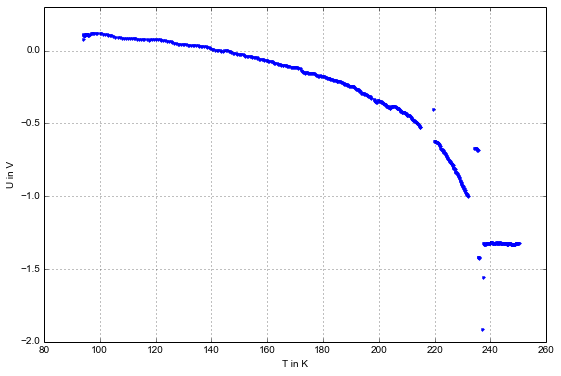
\includegraphics[width=0.6\textwidth]{abbildungen/Tb_sr_150.png}
\caption[Terbiumprobe senkrecht bei 15mT]{\textbf{Terbiumprobe senkrecht im Feld ($B = \SI{15}{mT}$) gekühlt, Rohdaten.} 
Das Magnetfeld am SQUID ist über die Temperatur aufgetragen. 
Da die Messwerte stark sprangen mussten die Unstetigkeiten nach Augenmaß korrigiert werden.
Insbesondere an der interessanten Stelle um die Curietemperatur traten viele Sprünge auf.}
\label{fig:Tb_sr_15}
\end{figure}




\begin{figure}
\centering
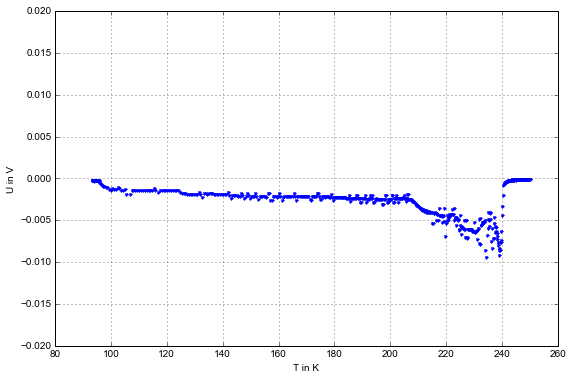
\includegraphics[width=0.6\textwidth]{abbildungen/Tb_sr_150_grad.png}
\caption[Terbiumprobe senkrecht bei Nullfeld]{\textbf{Terbiumprobe senkrecht im Feld ($B = \SI{15}{mT}$) gekühlt, geglättet und Gradient gebildet} 
Die Steigung des Magnetfeldes am SQUID ist über die Temperatur aufgetragen. 
Es ist ein Minimum zu erkennen und somit eine Curietemperatur ermittelbar.
Die Sprünge gestalteten die Auswertung dieses Minimums schwierig.}
\label{fig:Tb_sr_15_grad}
\end{figure}


\subsubsection{Terbiumprobe bei parallelem Einbau}

Die Terbiumprobe wurde mit zum Magnetfeld paralleler Ausrichtung auf den Probenhalter geschraubt. 
Ein Magnetfeld mit der vorgegebenen Feldstärke wurde angelegt und die Probe gekühlt.
Sobald die Probe auf die Temperatur des flüssigen Stickstoffs abgekühlt war,
wurde sie in den SQUID eingeführt.


\subsubsection*{Messung mit im Feld gekühlter Probe bei \SI{5}{mT}}

Außer einiger Abweichungen am Anfang der Messung ist der erwartete Verlauf in Abbildung \ref{fig:Tb_p_5} widergespiegelt.
Ein Minimum ist in der Steigung (Abb. ) eindeutig erkennbar und befindet sich an der Temperatur

\begin{equation}
T_{\mathrm{C}} = \SI{227}{\K} ~.
\end{equation}



\begin{figure}
\centering
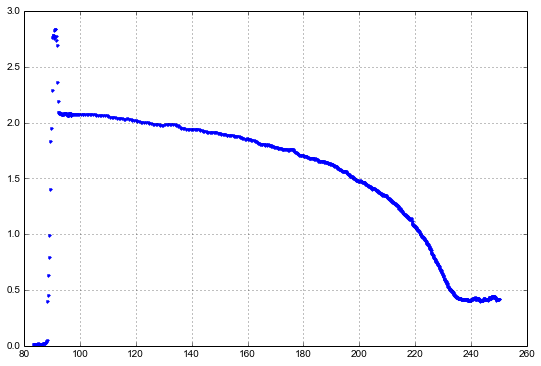
\includegraphics[width=0.6\textwidth]{abbildungen/Tb_p_5.png}
\caption[Terbiumprobe parallel bei 5mT]{\textbf{Terbiumprobe senkrecht im Feld ($B = \SI{5}{mT}$) gekühlt, Rohdaten.} 
Das Magnetfeld am SQUID ist über die Temperatur aufgetragen. }
\label{fig:Tb_p_5}
\end{figure}

\begin{figure}
\centering
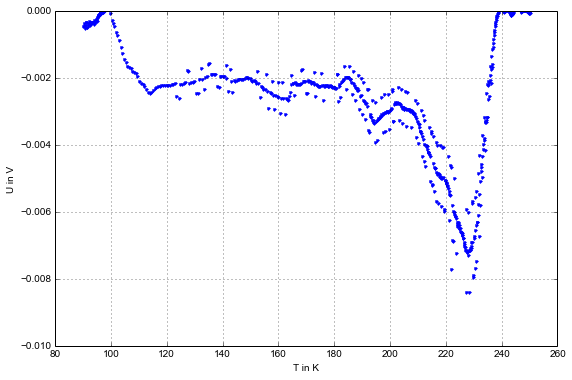
\includegraphics[width=0.6\textwidth]{abbildungen/Tb_p_5_grad.png}
\caption[Terbiumprobe parallel bei 5mT]{\textbf{Terbiumprobe senkrecht im Feld ($B = \SI{5}{mT}$) gekühlt, geglättet und Gradient gebildet} 
Die Steigung des Magnetfeldesam SQUID ist über die Temperatur aufgetragen. 
Es ist ein Minimum zu erkennen und somit eine Curietemperatur ermittelbar.
Alle Messwerte über $T =\SI{90}{K}$ wurden ausgeblendet.}
\label{fig:Tb_p_5_grad}
\end{figure}

\subsubsection*{Messung mit im Feld gekühlter Probe bei \SI{10}{mT}}

Der erwartete Verlauf in Abbildung \ref{fig:Tb_p_5} widergespiegelt.
Ein Minimum ist in der Steigung (Abb. ) eindeutig erkennbar und befindet sich an der Temperatur

\begin{equation}
T_{\mathrm{C}} = \SI{227}{\K} ~.
\end{equation}



\begin{figure}
\centering
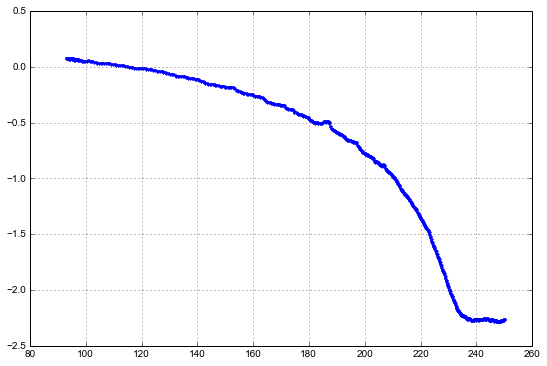
\includegraphics[width=0.6\textwidth]{abbildungen/Tb_p_10.png}
\caption[Terbiumprobe parallel bei 10mT]{\textbf{Terbiumprobe parallel im Feld ($B = \SI{10}{mT}$) gekühlt, Rohdaten.} 
Das Magnetfeld am SQUID ist über die Temperatur aufgetragen. }
\label{fig:Tb_p_10}
\end{figure}

\begin{figure}
\centering
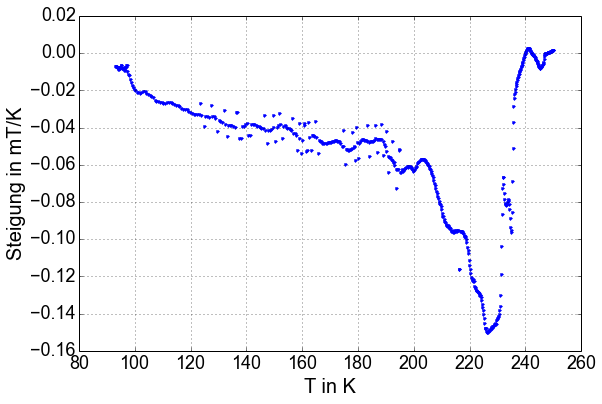
\includegraphics[width=0.6\textwidth]{abbildungen/Tb_p_10_grad.png}
\caption[Terbiumprobe parallel bei 10mT]{\textbf{Terbiumprobe parallel im Feld ($B = \SI{10}{mT}$) gekühlt, geglättet und Gradient gebildet} 
Die Steigung des Magnetfeldes am SQUID ist über die Temperatur aufgetragen. 
Es ist ein Minimum zu erkennen und somit eine Curietemperatur ermittelbar.}
\label{fig:Tb_p_10_grad}
\end{figure}


\subsubsection*{Messung mit im Feld gekühlter Probe bei \SI{15}{mT}}

Der erwartete Verlauf ist in Abbildung \ref{fig:Tb_p_5} dargestellt.
Ein Minimum ist in der Steigung (Abb. ) eindeutig erkennbar und befindet sich bei der Temperatur

\begin{equation}
T_{\mathrm{C}} = \SI{227}{\K} ~.
\end{equation}

\begin{figure}
\centering
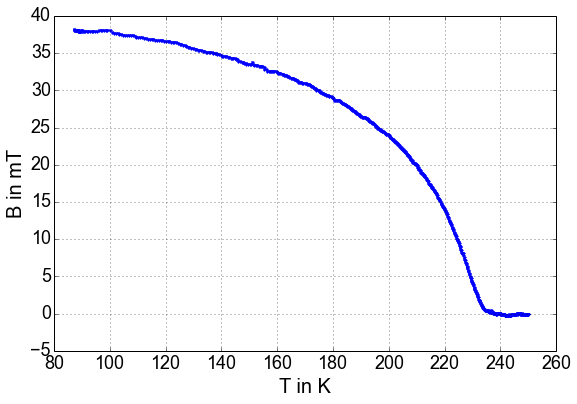
\includegraphics[width=0.6\textwidth]{abbildungen/Tb_p_15.png}
\caption[Terbiumprobe parallel bei 15mT]{\textbf{Terbiumprobe parallel im Feld ($B = \SI{15}{mT}$) gekühlt, Rohdaten.} 
Das Magnetfeld am SQUID ist über die Temperatur aufgetragen. }
\label{fig:Tb_p_15}
\end{figure}

\begin{figure}
\centering
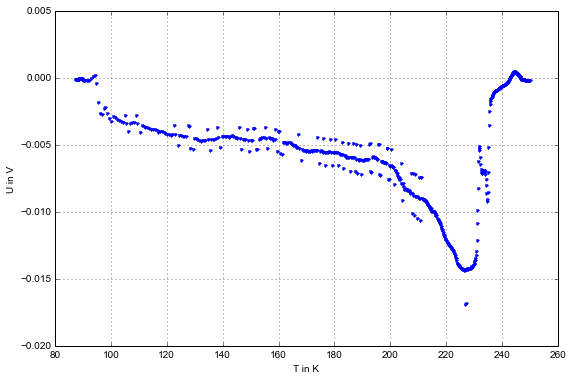
\includegraphics[width=0.6\textwidth]{abbildungen/Tb_p_15_grad.png}
\caption[Terbiumprobe parallel bei 15mT]{\textbf{Terbiumprobe parallel im Feld ($B = \SI{15}{mT}$) gekühlt, geglättet und Gradient gebildet} 
Die Steigung des Magnetfeldes am SQUID ist über die Temperatur aufgetragen. 
Es ist ein Minimum zu erkennen und somit eine Curietemperatur ermittelbar.}
\label{fig:Tb_p_15_grad}
\end{figure}


\clearpage
\subsubsection{Gadoliniumprobe}

\subsubsection*{Messung mit im Feld gekühlter Probe bei \SI{100}{mT}}

Die Gadoliniumprobe wurde eingebaut und bei angelegtem Feld mit einer Feldstärke von \SI{100}{mT} gekühlt.
Es wurde wieder während der Erwärmungsphase gemessen.
In Abbildung \ref{fig:Gadolinium} ist dies abgebildet.
Die Curietemperatur von \SI{292}{\K} ist zu erkennen.
Dies ist mit dem Literaturwert \SI{292.5}{\K} [\ref{ref:wiki},\ref{ref:mappe}] konsistent.
Eine weitere kritische Temperatur scheint bei \SI{231}{\K} zu sein.
Da Gadolinium selbst nicht supraleitend ist [\ref{ref:wiki}], 
handelt es sich dabei jedoch nicht um den Übergang des Gadoliniums in einen
supraleitenden Zustand.%ist eine Sprungtemperatur eher unwahrscheinlich.

\begin{figure}
\centering
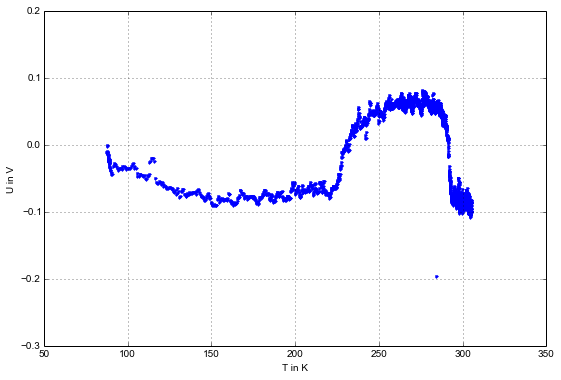
\includegraphics[width=0.6\textwidth]{abbildungen/gadolinium.png}
\caption[Gadolinium]{\textbf{Gadoliniumprobe parallel im Feld ($B = \SI{100}{mT}$) gekühlt.} 
Für sehr geringe Temperaturen zeigt sich ein flacher Verlauf auf Nullniveau.
Bei einer Temperatur von etwa \SI{231}{\K} steigt die Magnetisierung stark an und verweilt auf einem Plateau.
Wird die Curietemperatur von $T_{\mathrm{C}} = \SI{292}{\K}$ erreicht, fällt die Magnetisierung wieder auf Null ab.
} 
\label{fig:Gadolinium}
\end{figure}



\subsubsection{Vergleich}

Alle Curietemperaturen sind in Tabelle \ref{tab:vergleich} aufgelistet.
Die Werte für den parallelen Einbau sind konsistent.
Auch für den senkrechten Einbau weicht die Messung der im Feld gekühlten Probe nicht stark ab.
Bei den im Nullfeld gekühlten Messreihen konnten keine  Curietemperatur bestimmt werden.
Für das Nullfeld mit Magnetisierung bei tiefer Temperatur ist jedoch keine Curietemperatur erkennbar gewesen.
Gemittelt über alle Werte ergab sich die Curietemperatur von Terbium als
\begin{equation}
T_{\mathrm{C} }= \SI{229+-4}{\K} ~.
\end{equation}
Die Curietemperatur von \SI{230}{\K} [\ref{ref:wikitb}] liegt im Bereich der Messungenauigkeit.


\begin{table}[tb!]
\centering
\caption[Vergleich]{\textbf{Vergleich der Messergebnisse .} }
\begin{tabular}{cc}
\toprule
Probe	&	$T_{\mathrm{C}}$ in K	\\
\midrule
Tb, senkrecht ohne Magnetfeld &	- \\
Tb, senkrecht, Nullfeld mit Magnetisierung 	&	- \\
Tb, senkrecht, \SI{15}{mT}	&	235 \\
Tb, parallel, \SI{5}{mT}	&	227\\
Tb, parallel, \SI{10}{mT}	&	227\\
Tb, parallel, \SI{15}{mT}	&	227\\
Gd, \SI{1000}{mT} 	&	292\\
\bottomrule
\end{tabular}
\label{tab:vergleich}
\end{table}

\clearpage
\subsection{Neukurve}
Es sollte außerdem die Neukurve von Terbium (Tb) bei parallelem
Einbau bei einer festen, nicht zu hohen Temperatur, bestimmt werden.
Wir entschieden uns für eine Temperatur von $T = \SI{120}{\kelvin}$ und
zum Vergleich $T = \SI{180}{\kelvin}$.
Zum Erstellen der Kurve haben wir die Magnetisierungen bei diesen
Temperaturen aus den Magnetisierungskurven von parallel eingebautem
Terbium bei \SI{5}{\milli\tesla}, \SI{10}{\milli\tesla} und 
\SI{15}{\milli\tesla} ausgelesen, sowieo den Punkt (0|0) verwendet. 
Durch Auftragen der zur Magnetisierung verwendeten externen magnetischen Flussdichten 
gegen die durch Magnetisierung induzierte magnetische Flussdichte, die am SQUID gemessen wurde, 
erhielten wir die in Abbildung~\ref{fig:neukurve} zu sehenden Neukurvem.

\begin{figure}[tbh!]
  \centering
  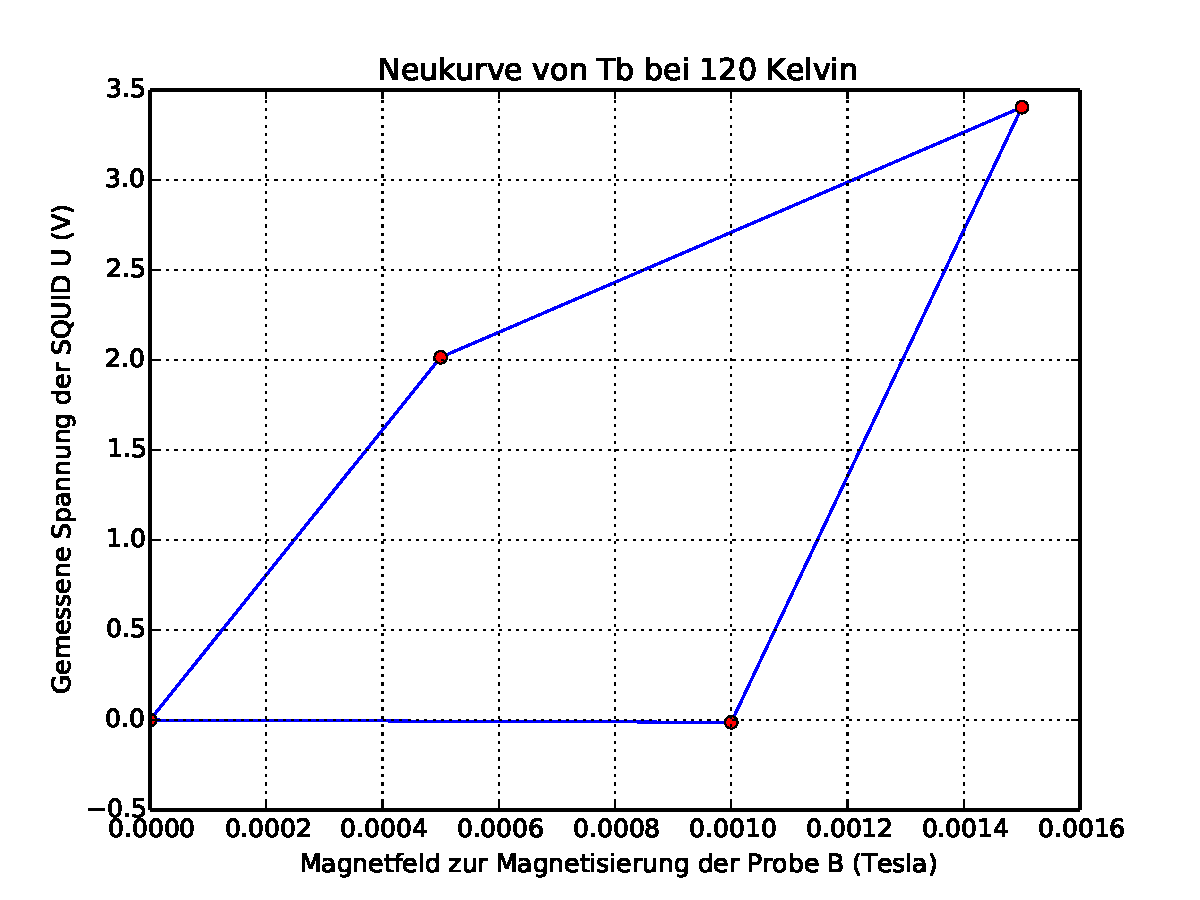
\includegraphics[width=0.6\textwidth]{abbildungen/neukurve.pdf}
  \caption{\textbf{Neukurve von Tb bei 120 Kelvin.} Zu sehen sind die
    die Messwerte als Punkte und Verbingungslinien zur besseren Veranschaulichung.}
  \label{fig:neukurve}
\end{figure}

Da wir mit dem Ursprung nur vier Messpunkte haben, daher lassen sich
damit nur ungefähre Aussagen treffen.
Es ist zu sehen, dass sich mit steigendem externen Magnetfeld auch die Magnetisierung in
der Probe entsprechend erhöht, was an einem steigenden gemessenen Magnetfeld am SQUID zu sehen ist.
Bei höheren externen Magnetfeldern $B_{\rm extern} > \SI{5}{\milli\tesla}$ wird die Erhöhung der Magnetisierung mit steigenden externen
Magnetfeld kleiner, was man auf Sättigungseffekte zurückführen könnte. 
Es wäre dabei jedoch ein Absinken der Steigung nach $B_{\rm extern} = \SI{10}{\milli\tesla}$ zu erwarten, was hier nicht der Fall ist.
Stattdessen bleibt die Steigung annähernd konstant. 
Eventuell könnte das an Ungenauigkeiten in der Messung liegen.
Jedoch haben wir zu wenige und zu ungenaue Messpunkte, um das genau sehen zu können. 
Vor allem wärem mehr Messpunkte bei noch höheren externen Magnetfeldern interessant, 
um genau sehen zu können, ob Sättigungseffekte eintreten.


 
\clearpage
\section{Quellen}
\begin{enumerate}
\item Vorbereitungsmappe.\label{ref:mappe}
\item \url{http://hydrogen.physik.uni-wuppertal.de/hyperphysics/hyperphysics/hbase/solids/squid.html} (18.1.2015).\label{ref:wuppertal}
\item \url{http://jsq.apps-1and1.net/category/information/what-is-a-squid/} (18.1.2015).
\item \url{http://de.wikipedia.org/wiki/Gadolinium} (\today)\label{ref:wiki}
\item \url{http://en.wikipedia.org/wiki/Terbium} (\today)\label{ref:wikitb}
\label{ref:jsq}
\end{enumerate}




\end{document}
